\documentclass[a4paper]{article}
\usepackage{graphicx}
\usepackage[comma]{natbib}
\usepackage{apalike} 
\setcitestyle{aysep={,}}
\usepackage{amsmath, amsthm, amsfonts, amssymb, amscd, bm, breqn}
\usepackage{dsfont}
\usepackage{verbatim}
\usepackage{url}
\usepackage[hidelinks]{hyperref}
\usepackage[table,xcdraw]{xcolor}
\usepackage{float}
\usepackage{enumerate}
\usepackage{enumitem}
\usepackage[noabbrev,capitalize]{cleveref}
\usepackage[font=footnotesize,labelfont=bf,width=0.8\textwidth]{caption}
\usepackage{subcaption}
\usepackage{upgreek}


% !TeX spellcheck = en_GB

%\textwidth = 6.2 in≠
\textheight = 9 in
\topmargin = 0.0 in
	\addtolength{\oddsidemargin}{-.575in}
	\addtolength{\evensidemargin}{-.575in}
	\addtolength{\textwidth}{1.15in}
%\headheight = 0.0 in
%\headsep = 0.0 in
\parskip = 0.1in
% \parindent = 0.2cm

\newcommand{\N}{\mathbb{N}}
\newcommand{\R}{\mathbb{R}}
\newcommand{\Z}{\mathbb{Z}}
\newcommand{\Q}{\mathbb{Q}}
\newcommand{\bs}[1]{\boldsymbol{#1}}
\newcommand{\y}{\boldsymbol{y}}
\renewcommand{\d}{\text{d}}

% \newcommand\numberthis{\addtocounter{equation}{1}\tag{\theequation}}

\begin{document}

% \title{Ellipsoid Criterion}
\title{Locust Analysis Summary}
\author{Oliver Lountain}

\maketitle


% \tableofcontents


\section{Introduction}

In this analysis we have aimed to connect the input parameters of a simulation of locust dynamics to the qualitatively different shapes that these swarms can take. Specifically, we have aimed to predict shape based upon input parameters. We are interested in classifying a swarm into one of the following shapes:
\begin{itemize}
    \item comet,
    \item compact,
    \item fan,
    \item stream,
    \item column, and, if a swarm cannot be placed into one of these categories,
    \item other.
\end{itemize}



\section{Labelling the Shape of a Simulation}

In order to predict shape based on input parameters, we first needed to obtain a data set containing input parameters and the corresponding shape of the swarm for a number of simulation runs. Since the number of simulations is large, we first needed to develop a model to assign a shape to a swarm based on the locations of the locusts at the end of the simulation. To quantitatively measure the shape based on these locations, we considered a number of different summary statistics.

\subsection{Summary Statistics}

We have used a number of summary statistics to quantitatively describe the shape of the locust swarms. The statistics were chosen to capture the qualitative differences that can be observed in the distinct swarms, and in many cases simple statistics were used to maintain interpretability. Each statistic was computed on the swarm of locusts that were present at the end of the simulation. 

\subsubsection{Ratio of x-spread to y-spread}

The first statistics that was used was the ratio of the x-spread to the y-spread of the swarm. That is, the distance between the smallest and largest x-coordinates of the locusts in the swarm, divided by the distance between the smallest and largest y-coordinates of the locusts in the swarm. The motivation for this arose from the clear distinction that could be seen between fan-shaped swarms, in which the y-spread was greater than the x-spread; comets, in which the x-spread was slightly greater than the y-spread; and streams and columns, in which the x-spread was substantially greater than the y-spread.

\subsubsection{Number of Occupied Squares}

The number of occupied squares was used as a measure of the total spread of the swarm. This could be used to distinguish the swarms which had all locusts concentrated in a small number of grid squares from those which were more spread out.

\subsubsection{Skewness of Density Distribution}

The skewness of the density distribution was used to distinguish the swarms which had a more even distribution of locusts than those which had locusts concentrated at the front or back of the swarm. In retrospect, it may have been better to look at the skewness of the density of x and y coordinates separately, or possibly just the x-coordinates.

\subsubsection{Fractal Dimension}

The fractal dimension of the swarm was also calculated. This was a less interpretable statistic but was investigated as it had been used in previous analysis. In the end it was used as it seemed to be a useful predictor in the model. 


{\color{red}{Show some plots of two statistics against one another coloured by class.}}

\subsection*{Unused Summary Statistics}

\subsubsection{Proportion of Squares Containing a Threshold Number of Locusts}

This was investigated as another measure of how spread out the swarm was. However, we found that this was significantly correlated with the number of occupied grid squares, and so was not used.

\subsubsection{Rotation Determined by PCA}

The rotation of the swarm in 2-D space was considered, though it was found that the rotation was almost always very close to zero, as the simulation had been designed to correct for any changes in direction.

\subsubsection{Persistent Homology}

{\color{red}{Include some persistence diagrams to show qualitatively how well this performs.}}

\subsection{Training a Model}

To use these summary statistics to predict the shape of a swarm, we trained a random forest. The training and testing set was obtained by manually labelling a subset of the simulations. This model was found to have 100\% accuracy on the testing set (this can be seen in the script 04\_label\_all\_data.R), and was then applied to the unlabelled simulations. To validate the model, we took a sample of the now-labelled simulations, and manually verified whether the labels were correct. This produced a new set of training data which was added to the existing set, and the model was trained again. Performance could be improved further by repeating this process.

We note that since, for every combination of input parameters, the simulation was repeated 20 times, it is possible that any given parameter combination could receive different label on different runs. In particular, we note that only in 76.9\% of the unique combinations of parameters, did each of the 20 simulation runs receive the same label (this can be seen in the script 05\_check\_labels\_within\_param\_combos.R). Such instances result in the random forest described in the next section having proportions less than one assigned to parameter combinations when treated as predictor variables.


\section{Predicting Shape from Simulation Parameters}

The next step in the process of predicting swarm shape from simulation parameters was to use the label the entire set of simulation runs using the first model, and then treat this labelled data set as the ground truth. We then used the parameters as predictor variables and trained a second random forest on this data set.

\subsection{Model Performance}

We found that the model predicted class correctly with 90.9\% accuracy (this can be seen in the script 04\_label\_all\_data.R). However, it is worth noting that this measurement of accuracy assumes that the initial labelling based on summary statistics was done perfectly. Also, the model performed worst on the other class, in particular incorrectly predicting a different label for swarms which truly belonged to the other class. This can be seen in the confusion matrix below:

{\color{red}{INSERT CONFUSION MATRIX}}

{\color{red}{include variable importance}}

\begin{figure}[]
	\centering
	\includegraphics[width=1\linewidth]{../Analysis/Plots/DALEX/dalex_analysis_vip.png}
	\caption{VIP}
	\label{fig:vip}
\end{figure}

{\color{red}{Include some plots of fa against jumpD at different fixed values of other parameters.}}

{\color{red}{Include PCA biplots}}

\begin{figure}[]
	\centering
	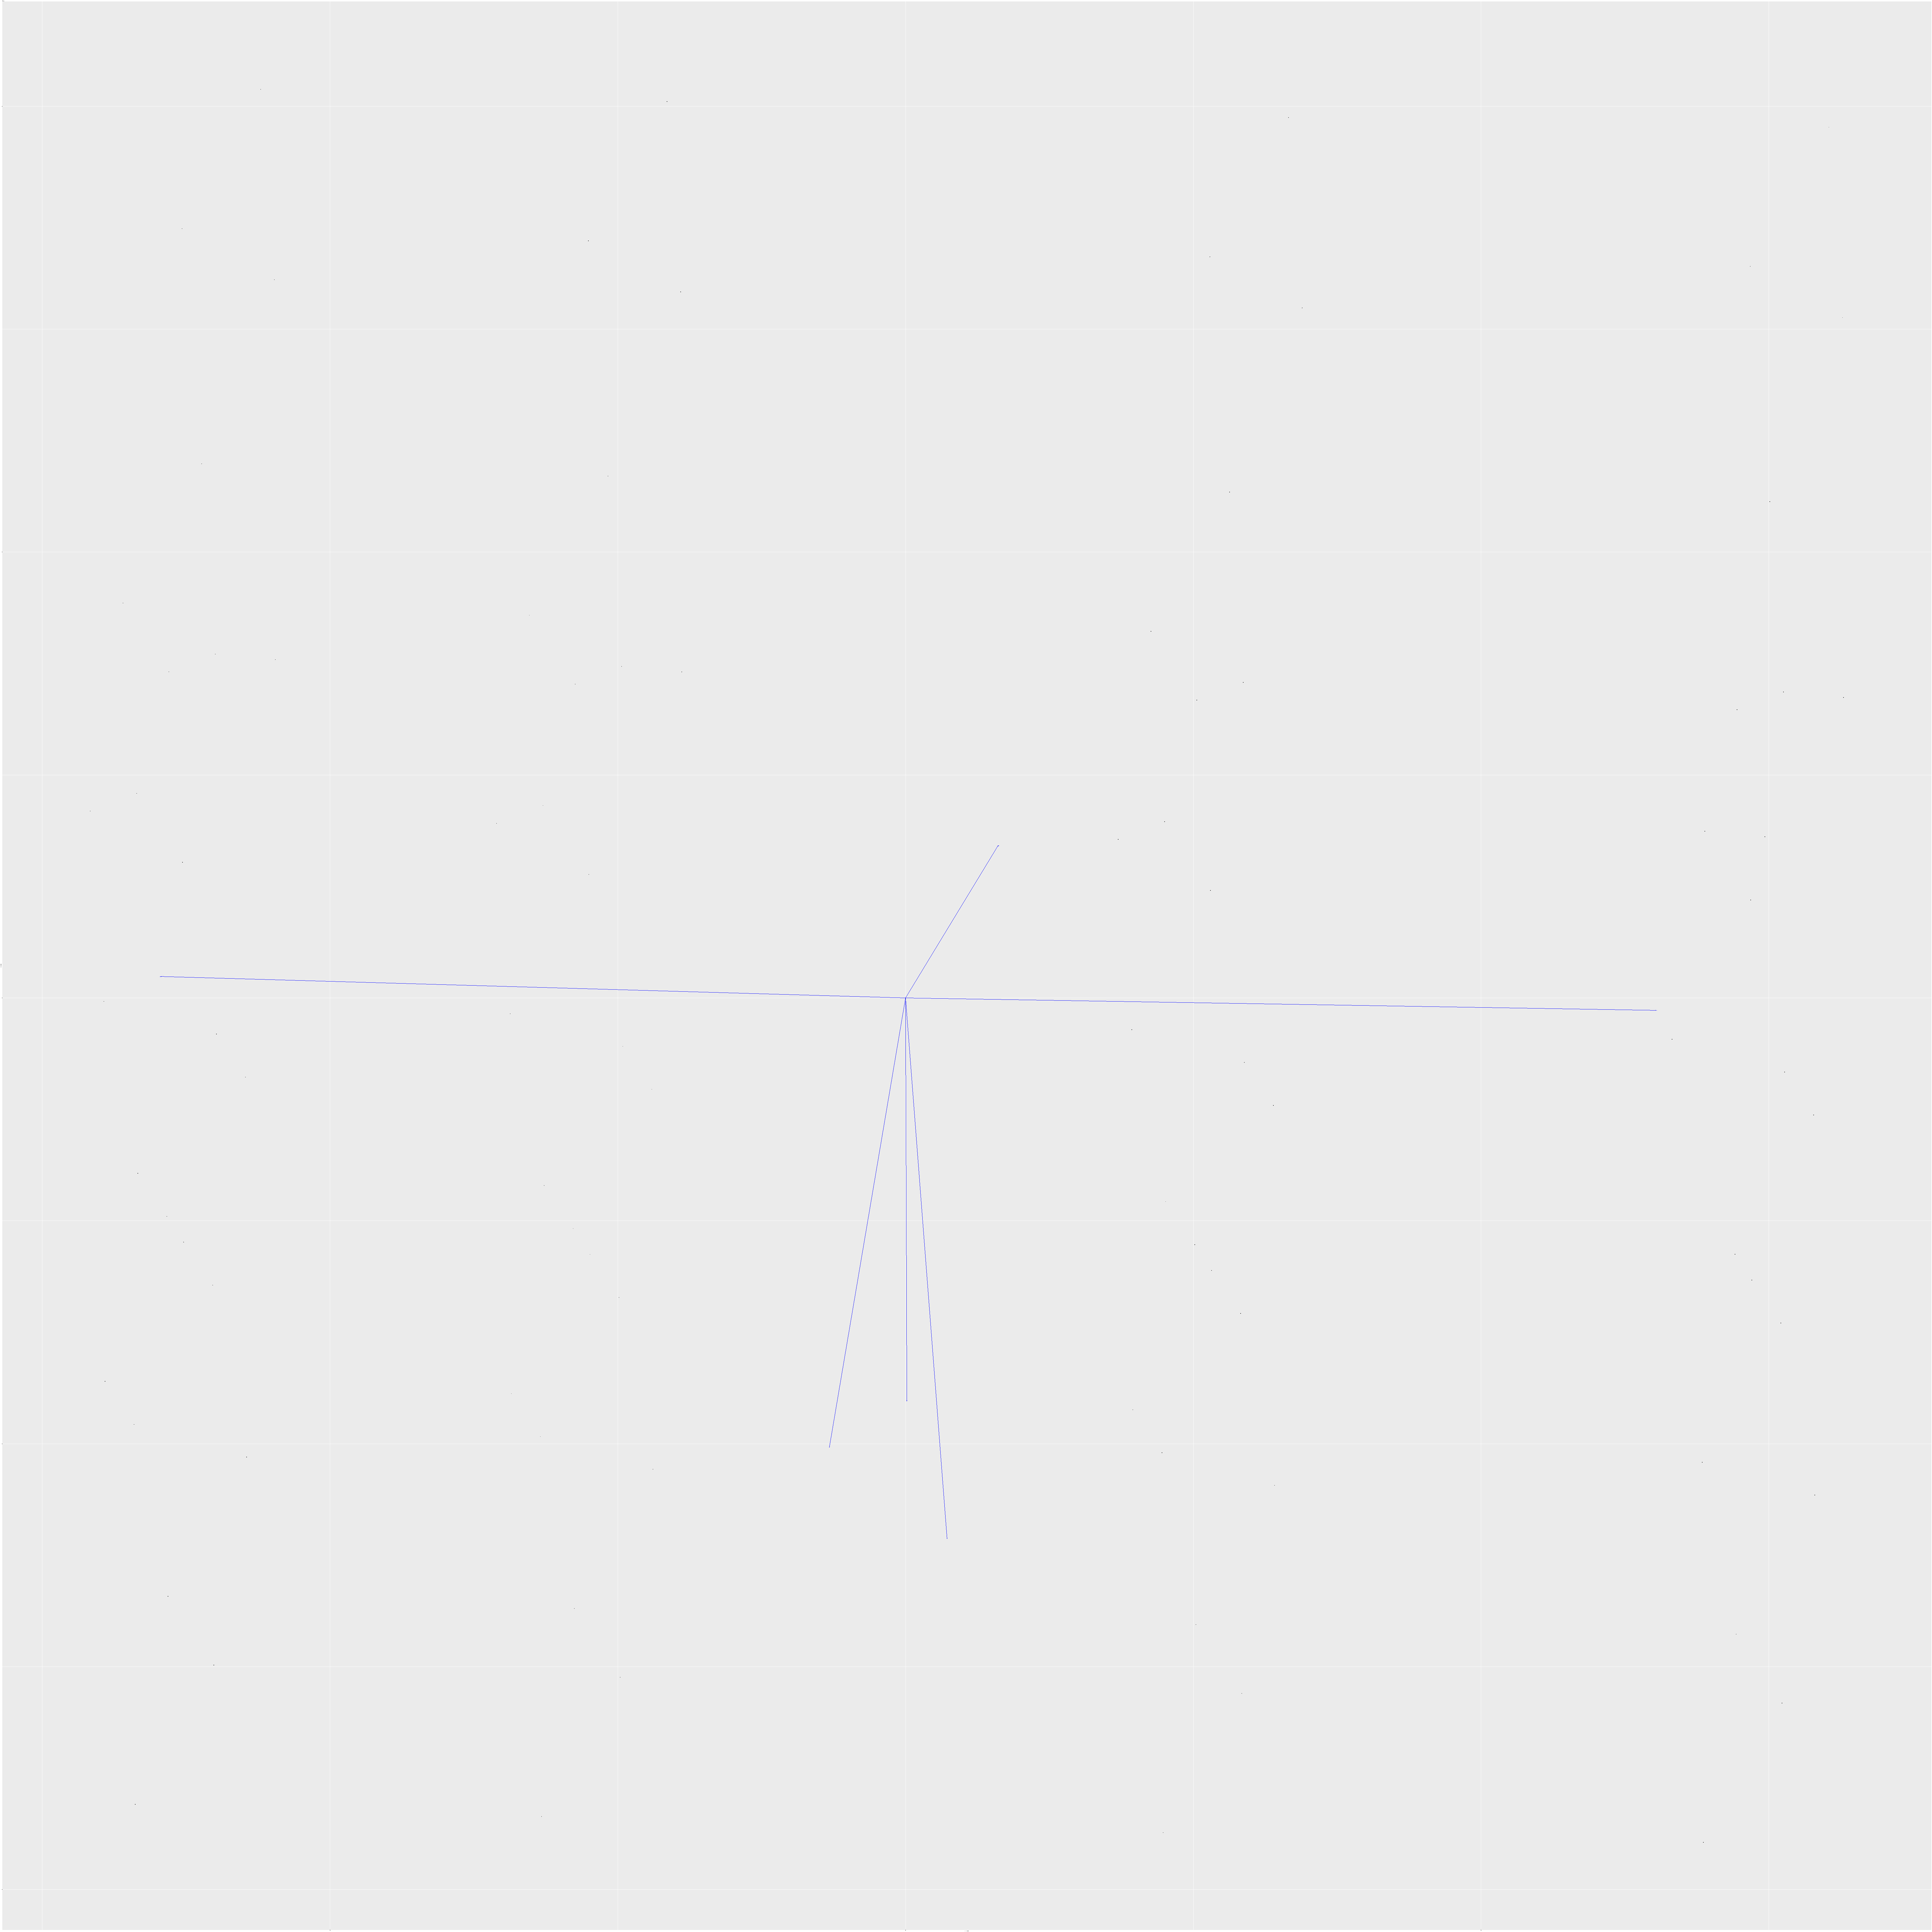
\includegraphics[width=1\linewidth]{../Analysis/Plots/PCA/pca_of_parameters_comet_biplot.eps}
	\caption{VIP}
	\label{fig:biplot}
\end{figure}



\section{Discussion}

\end{document}